\documentclass{article}
\usepackage[a4paper, total={7in, 8in}]{geometry}
\usepackage{spverbatim}
\usepackage{minted}
\usepackage{amssymb}
\usepackage{bm}
\usepackage{graphicx}
\usepackage{amsmath}


\title{Homework 2: EECE 5639 - Computer Vision}
\author{Sreejith Sreekumar: 001277209}
\date{\today}


\begin{document}

\maketitle

\section{Question 1}

\subsection{Code}
\begin{minted}{matlab}

function gray_img = grayscale_generator(w,h)  
    gray_img = im2double(128 * ones(w,'uint8'));
end

function sigma = estimate_noise(ImageArray, width, height, count)

    % calculation of E(i,j)
    E = double(zeros(height,width));
    %E = im2double(E)

    for k = 1:count
        for i = 1:width
            for j = 1:height
                E(i,j) = E(i,j) + double(ImageArray(k).Image(i,j));
            end
        end
    end

    E = 1/count * E;
    
    % calculation of standard deviation of E(i,j)
    sum_sq_diff = 0
    
    for k = 1:count
        for i = 1:width
            for j = 1:height
                sum_sq_diff = sum_sq_diff + (E(i,j) - double(ImageArray(k).Image(i,j)))^2;
            end
        end
    end
    
    sigma = sqrt(((1/(count -1)) * sum_sq_diff))
    
end

count = 10;
width = 256;
height = 256;


% 10 grayscale images and store in a stucture
ImgArray(1:count) = struct('Image', [], 'Label', '');
for j = 1:count
  ImgArray(j).Image = grayscale_generator(width, height);
  ImgArray(j).Label = j;
end

% add additive zero-mean Gaussian noise to all those images
variance = (2*2)/(255*255)
for j = 1:count
    ImgArray(j).Image = imnoise(ImgArray(j).Image,'gaussian', 0, variance);
end

noise = estimate_noise(ImgArray, width, height, count);
disp("Estimated noise in the images: " + noise)
    
\end{minted}


\subsection{Results}

\begin{minted}{matlab}
variance =

   6.1515e-05


sum_sq_diff =

     0


sigma =

    2.0071

Estimated noise in the images: 2.0071

\end{minted}  


\subsection{Comments}
Grayscale images are generated and are stored in a structure arrray. The structure contains the content of the image as a matrix and a label (an integer).
Zero mean gaussian noise with a varience of 2.0 is added to every image in the array.

Using the EST\_NOISE procedure, the estimated gaussian noise in the image array is around 2.00



\section{Question 2: Box Filter}

\subsection{Code}
\begin{minted}{matlab}
filterSize = 3;
for j = 1:count
    ImgArray(j).Image = imboxfilt(ImgArray(j).Image, filterSize);
end

% use the function implemented for question 1
noise = estimate_noise(ImgArray, width, height, count);
disp("Estimated noise in the images: " + noise)
\end{minted}

\subsection{Results}

\begin{minted}{matlab}
sum_sq_diff =

     0


sigma =

    0.6733

Estimated noise in the images: 0.67326  
\end{minted}  

\subsection{Comments}
Upon applying the 3 x 3 box filter, the noise reduces from 2.00 to 0.67



\section{Question 3}


\subsection{Code: Generating the 2D gaussian filter mask}
\begin{minted}{matlab}

hsize = 7;
sigma = 1.4;
gaussian_filter = fspecial('gaussian',hsize,sigma)
\end{minted}

\subsection{Result}
\begin{minted}{matlab}
gaussian_filter =

    0.0008    0.0030    0.0065    0.0084    0.0065    0.0030    0.0008
    0.0030    0.0108    0.0232    0.0299    0.0232    0.0108    0.0030
    0.0065    0.0232    0.0498    0.0643    0.0498    0.0232    0.0065
    0.0084    0.0299    0.0643    0.0830    0.0643    0.0299    0.0084
    0.0065    0.0232    0.0498    0.0643    0.0498    0.0232    0.0065
    0.0030    0.0108    0.0232    0.0299    0.0232    0.0108    0.0030
    0.0008    0.0030    0.0065    0.0084    0.0065    0.0030    0.0008
    
\end{minted}  

Separating into a horizontal and a vertical filter by the formula:

\[
  f(x, y) = (\frac{1}{\sqrt{K}} e^{- \frac{x^{2}} {2 \sigma^{2}} }) (\frac{1}{\sqrt{K}} e^{- \frac{y^{2}} {2 \sigma^{2}} })
  \]

\[
  f(x, y) = (\frac{1}{\sqrt{K}} e^{- \frac{x^{2}}{3.28}}) (\frac{1}{\sqrt{K}} e^{- \frac{y^{2}} {3.28}})
\]

\[
X = [0.0008\    0.0030\    0.0065\    0.0084\    0.0065\    0.0030\    0.0008]\ and\ Y = X^{T}
\]

Scaling this, we've:

\[
X = \frac{1}{36} [1\    4\     8\    10\    8\    4\    1]\ and\  Y = X^{T}
\]

\pagebreak

\begin{figure}
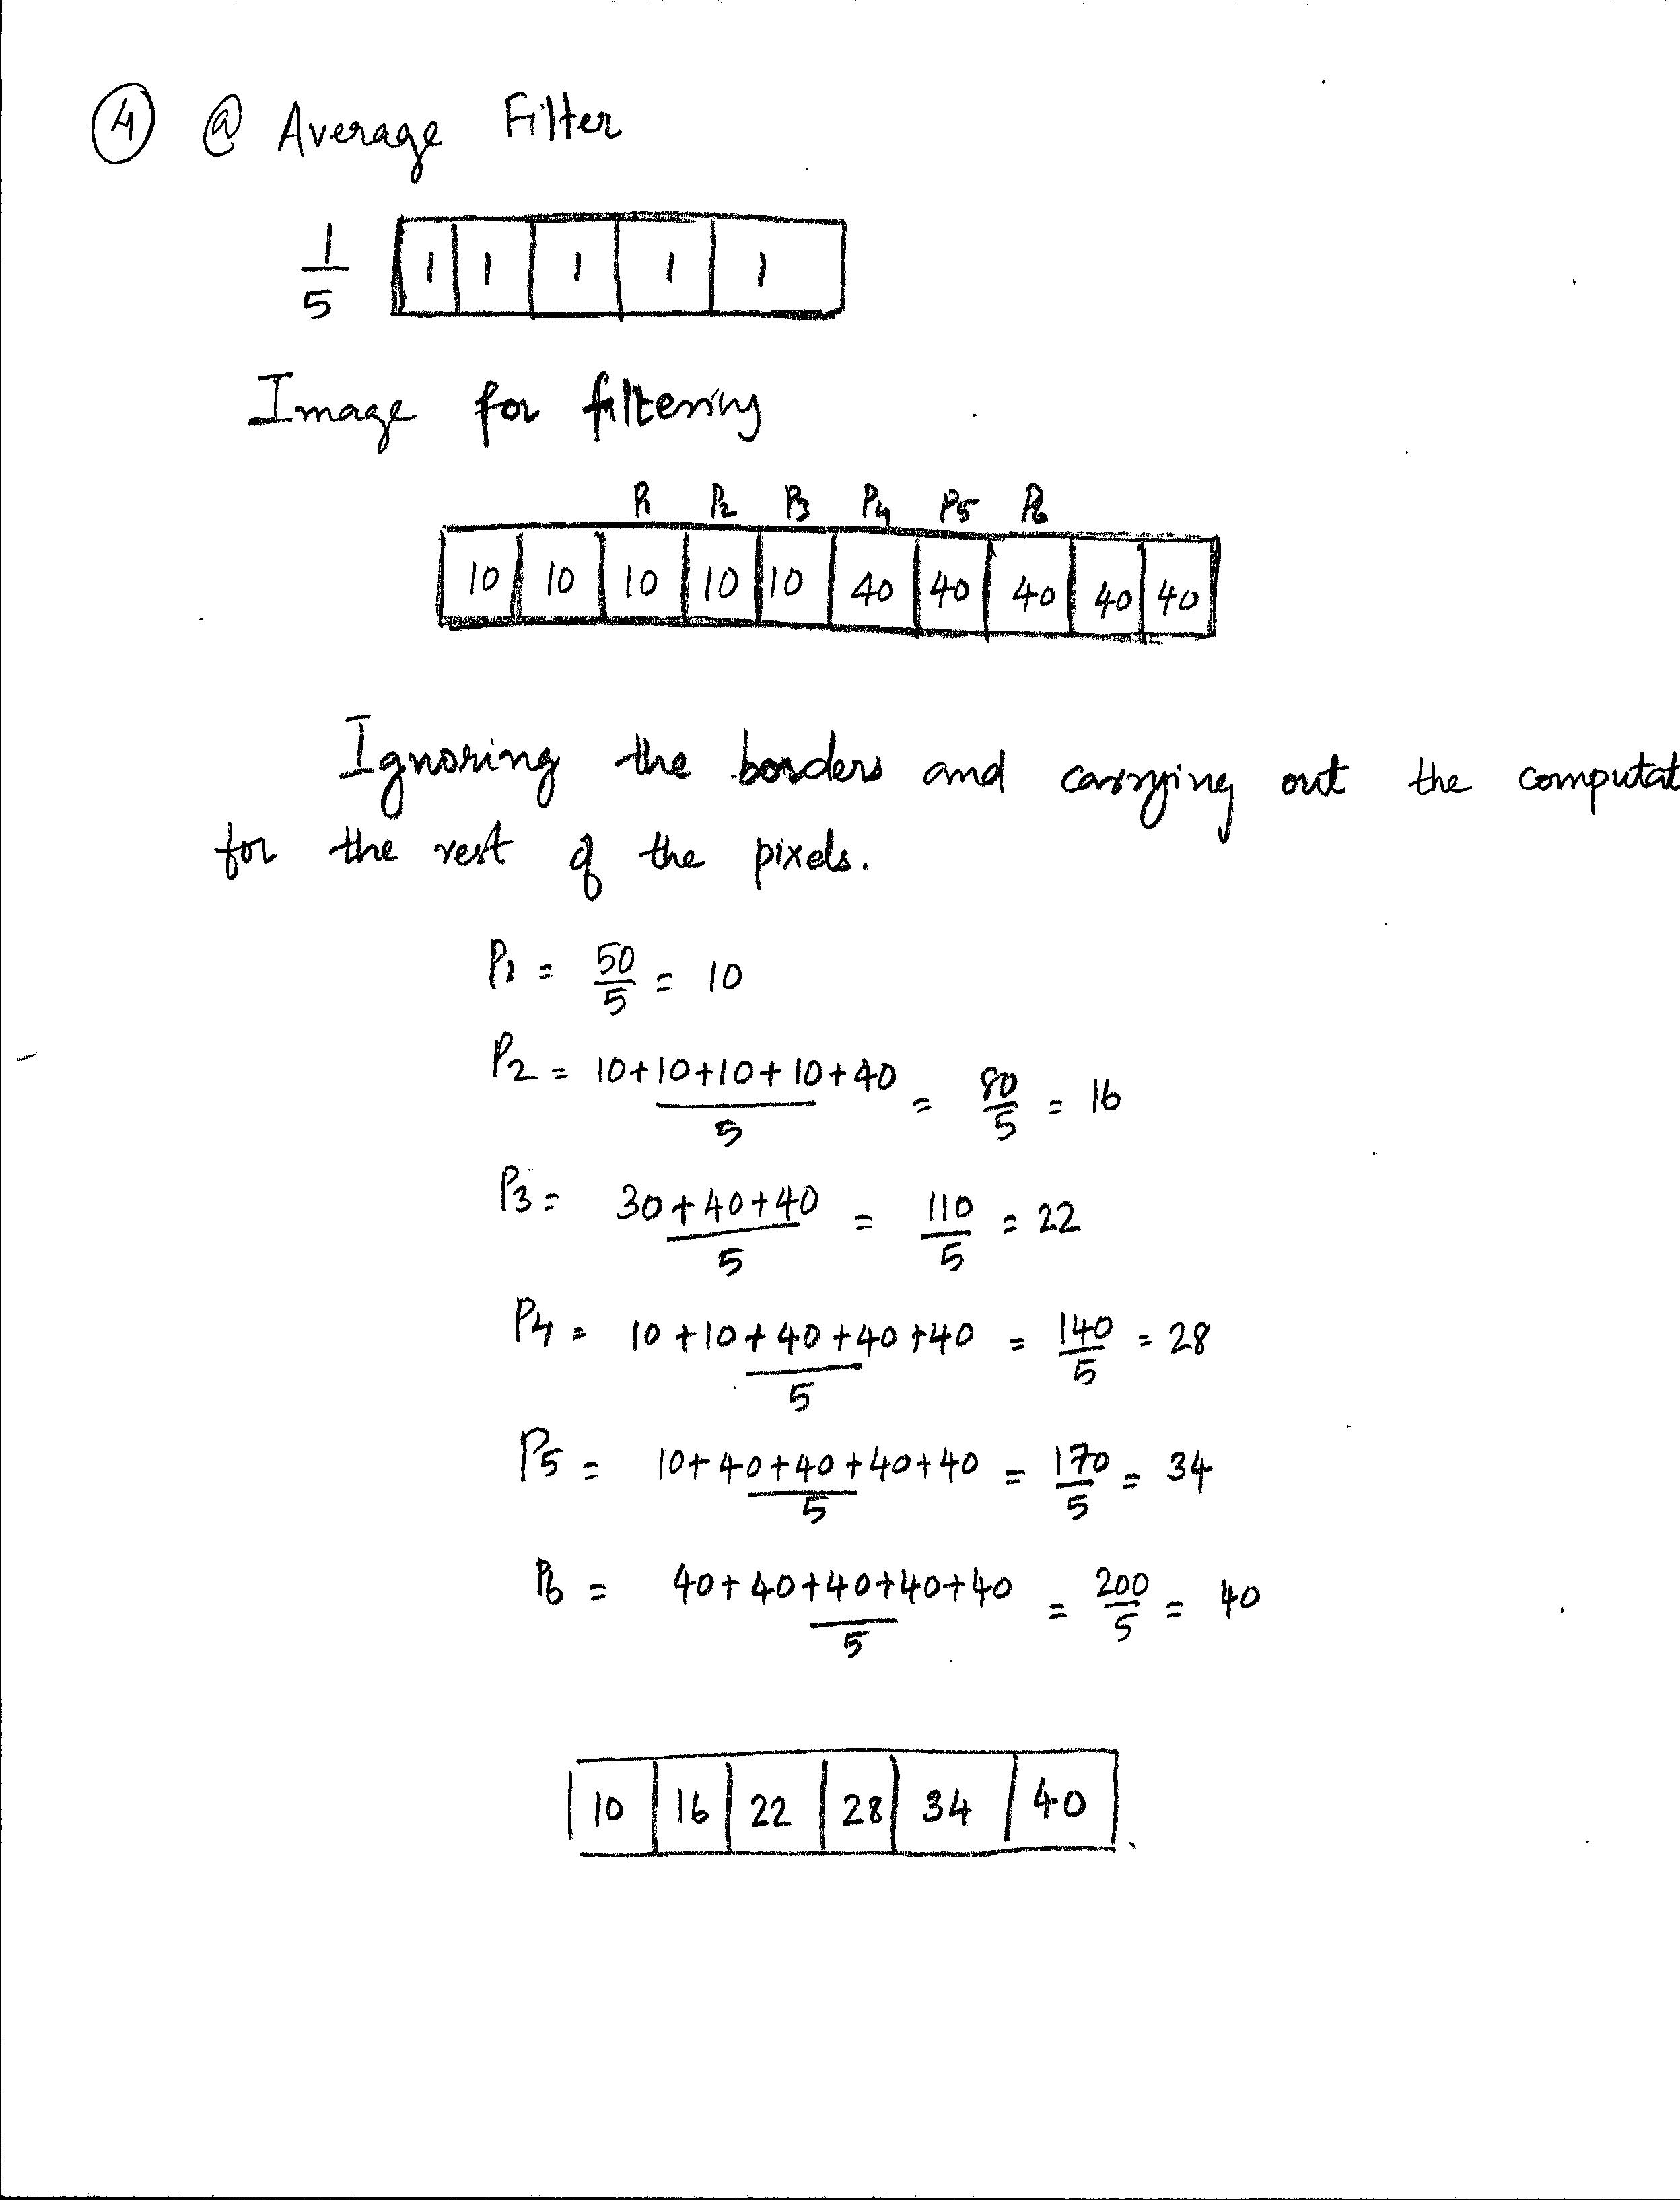
\includegraphics[width=15cm]{1.jpg}
\end{figure}

\begin{figure}
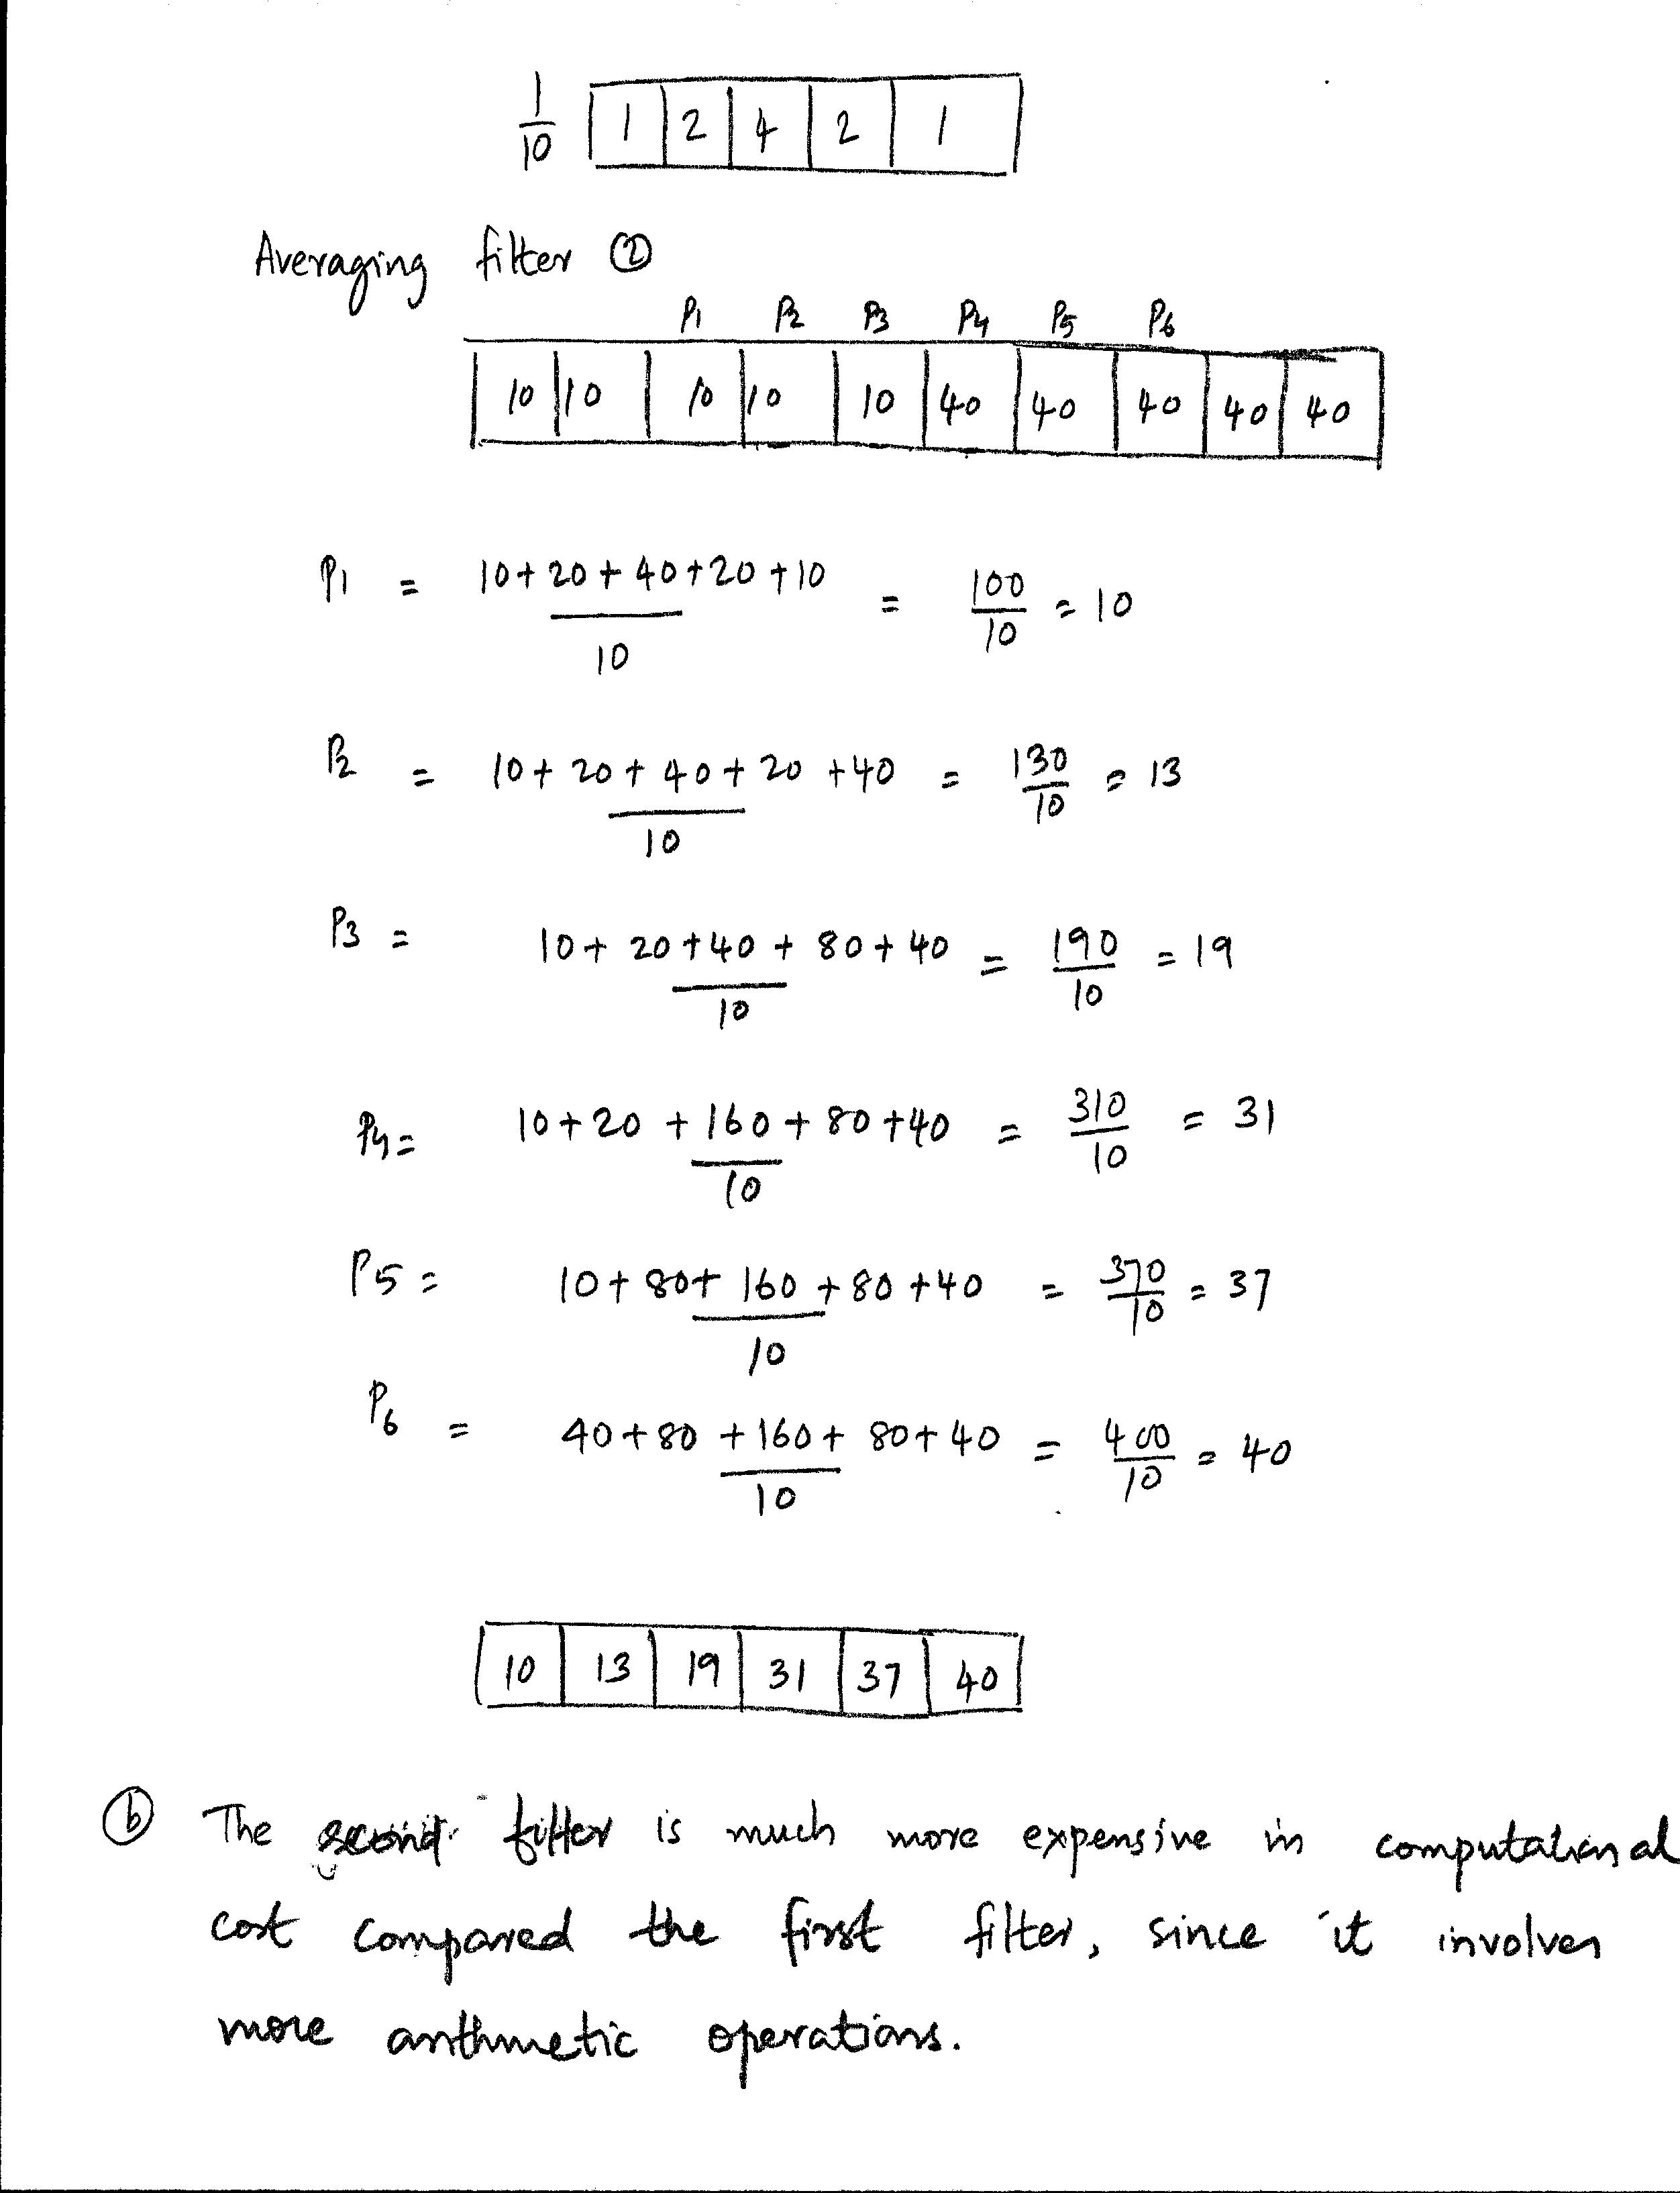
\includegraphics[width=15cm]{2.jpg}
\end{figure}

\begin{figure}
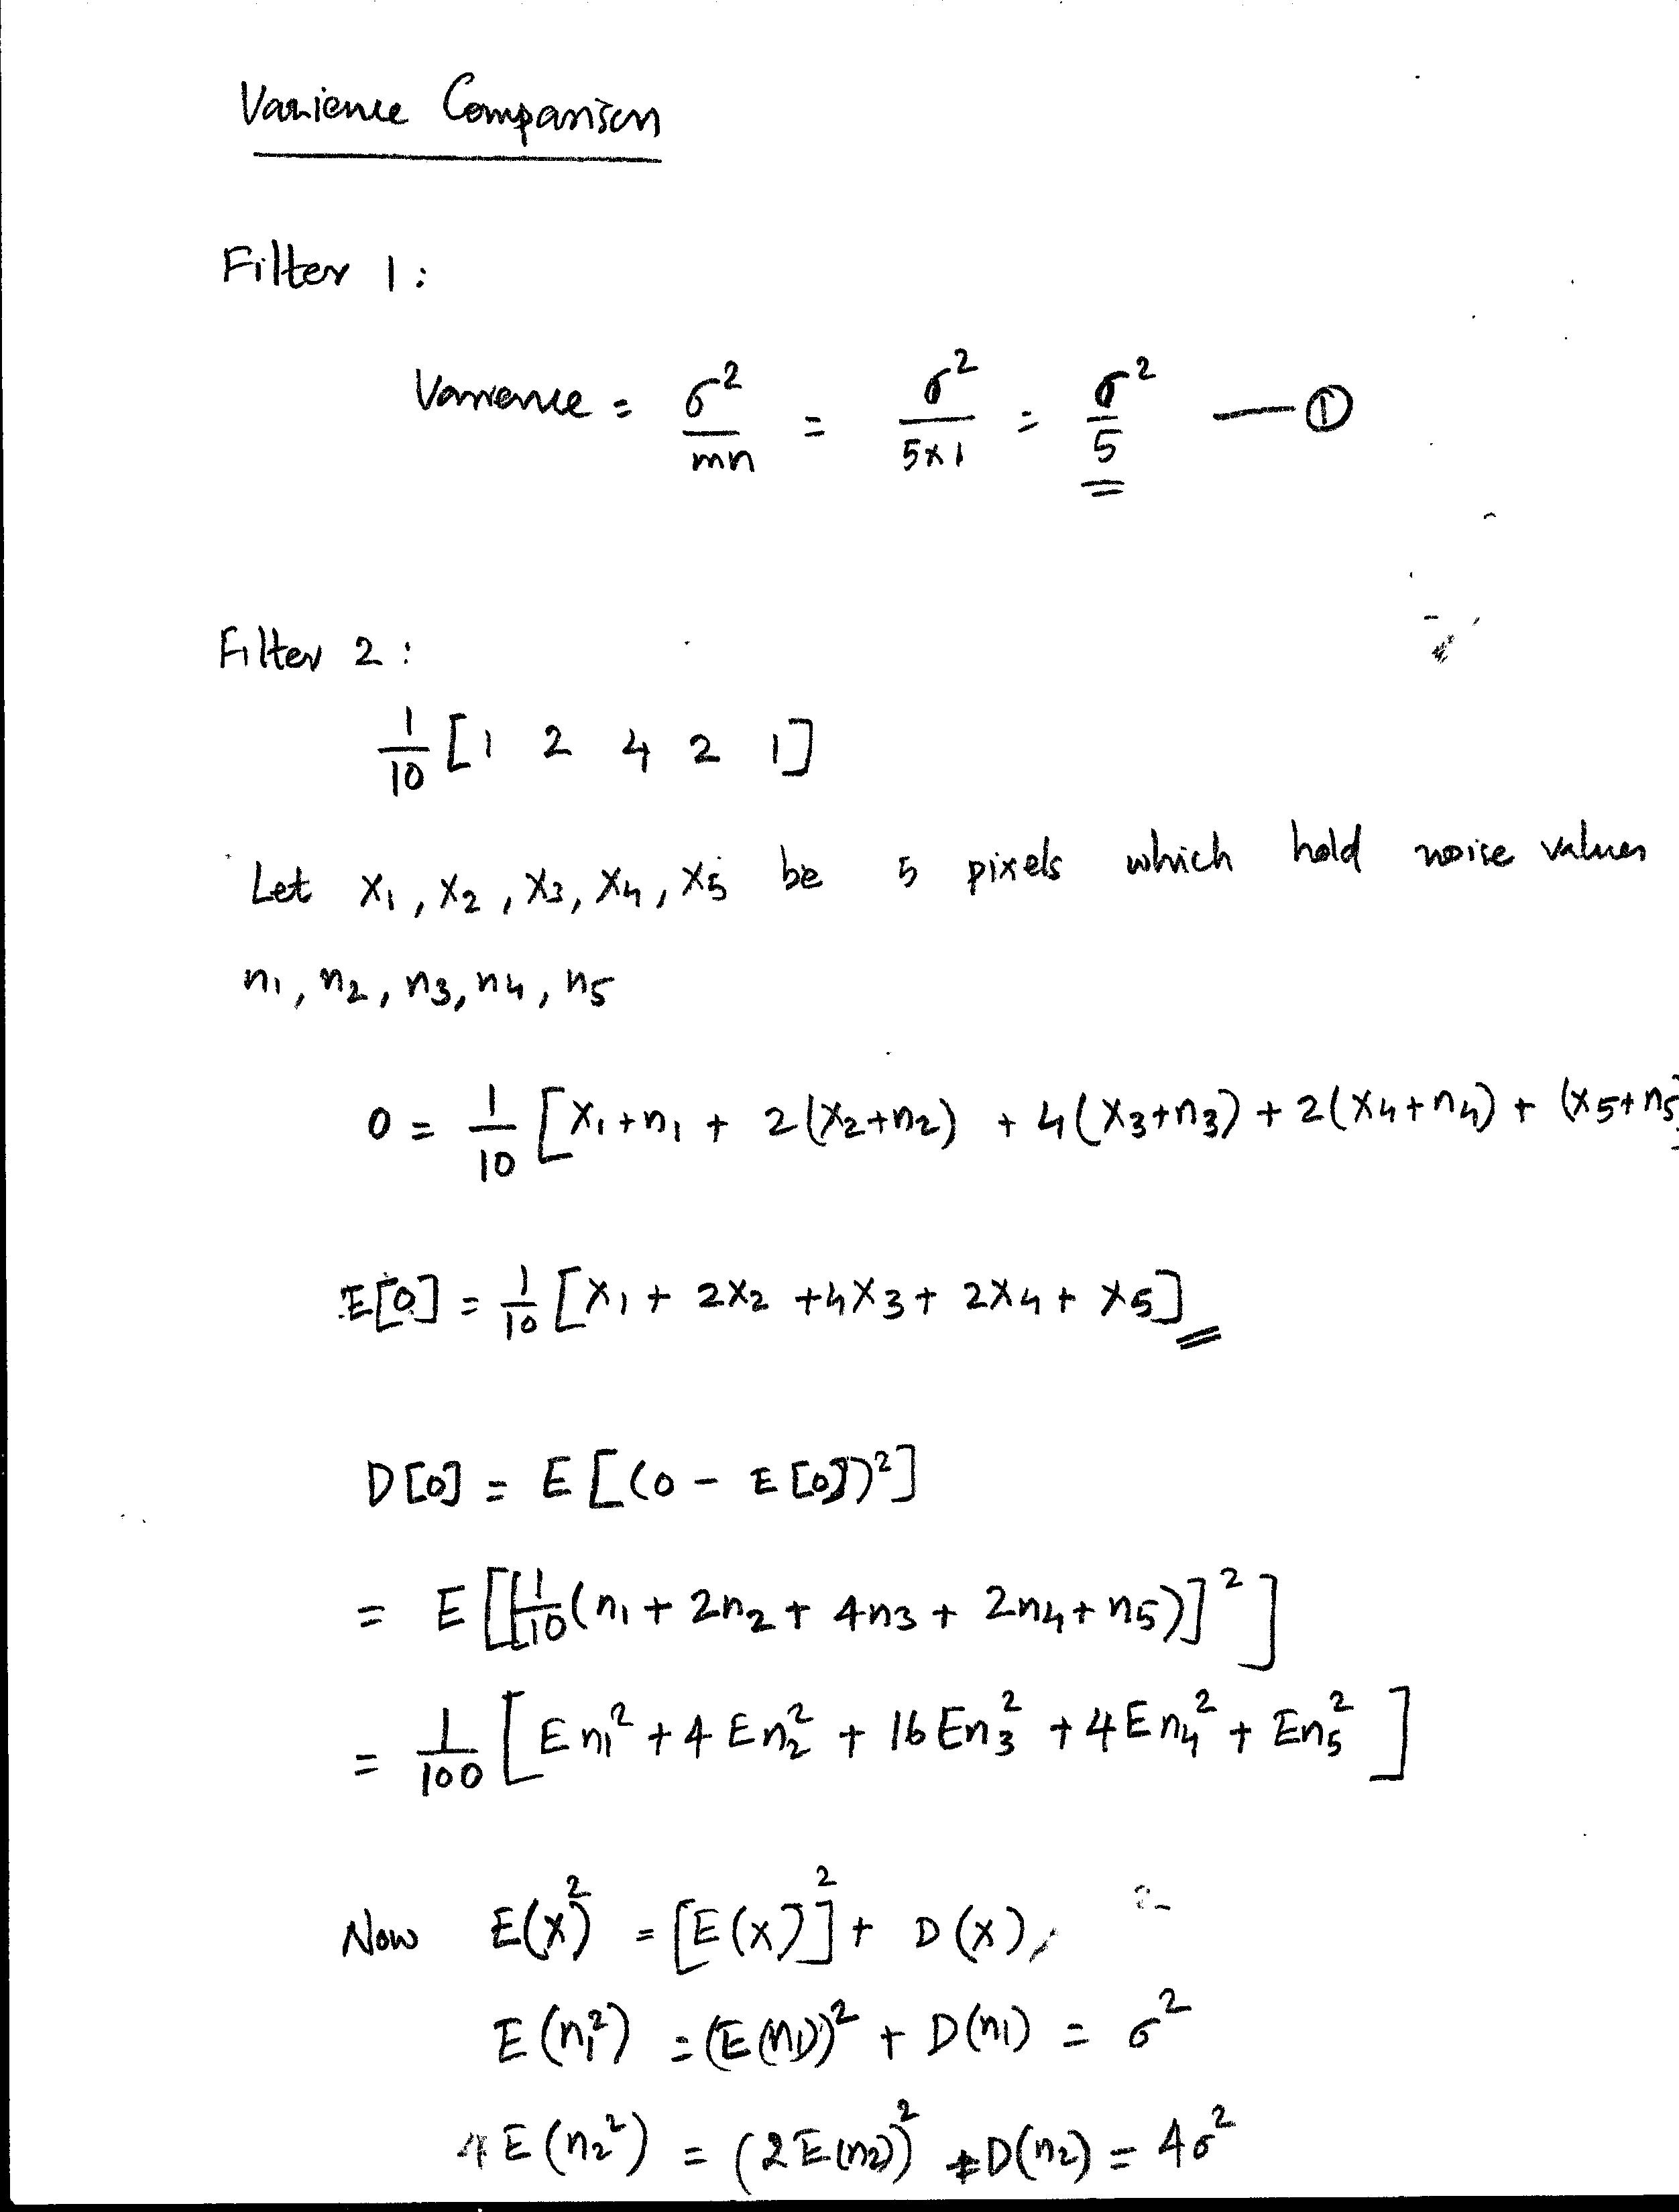
\includegraphics[width=15cm]{3.jpg}
\end{figure}

\begin{figure}
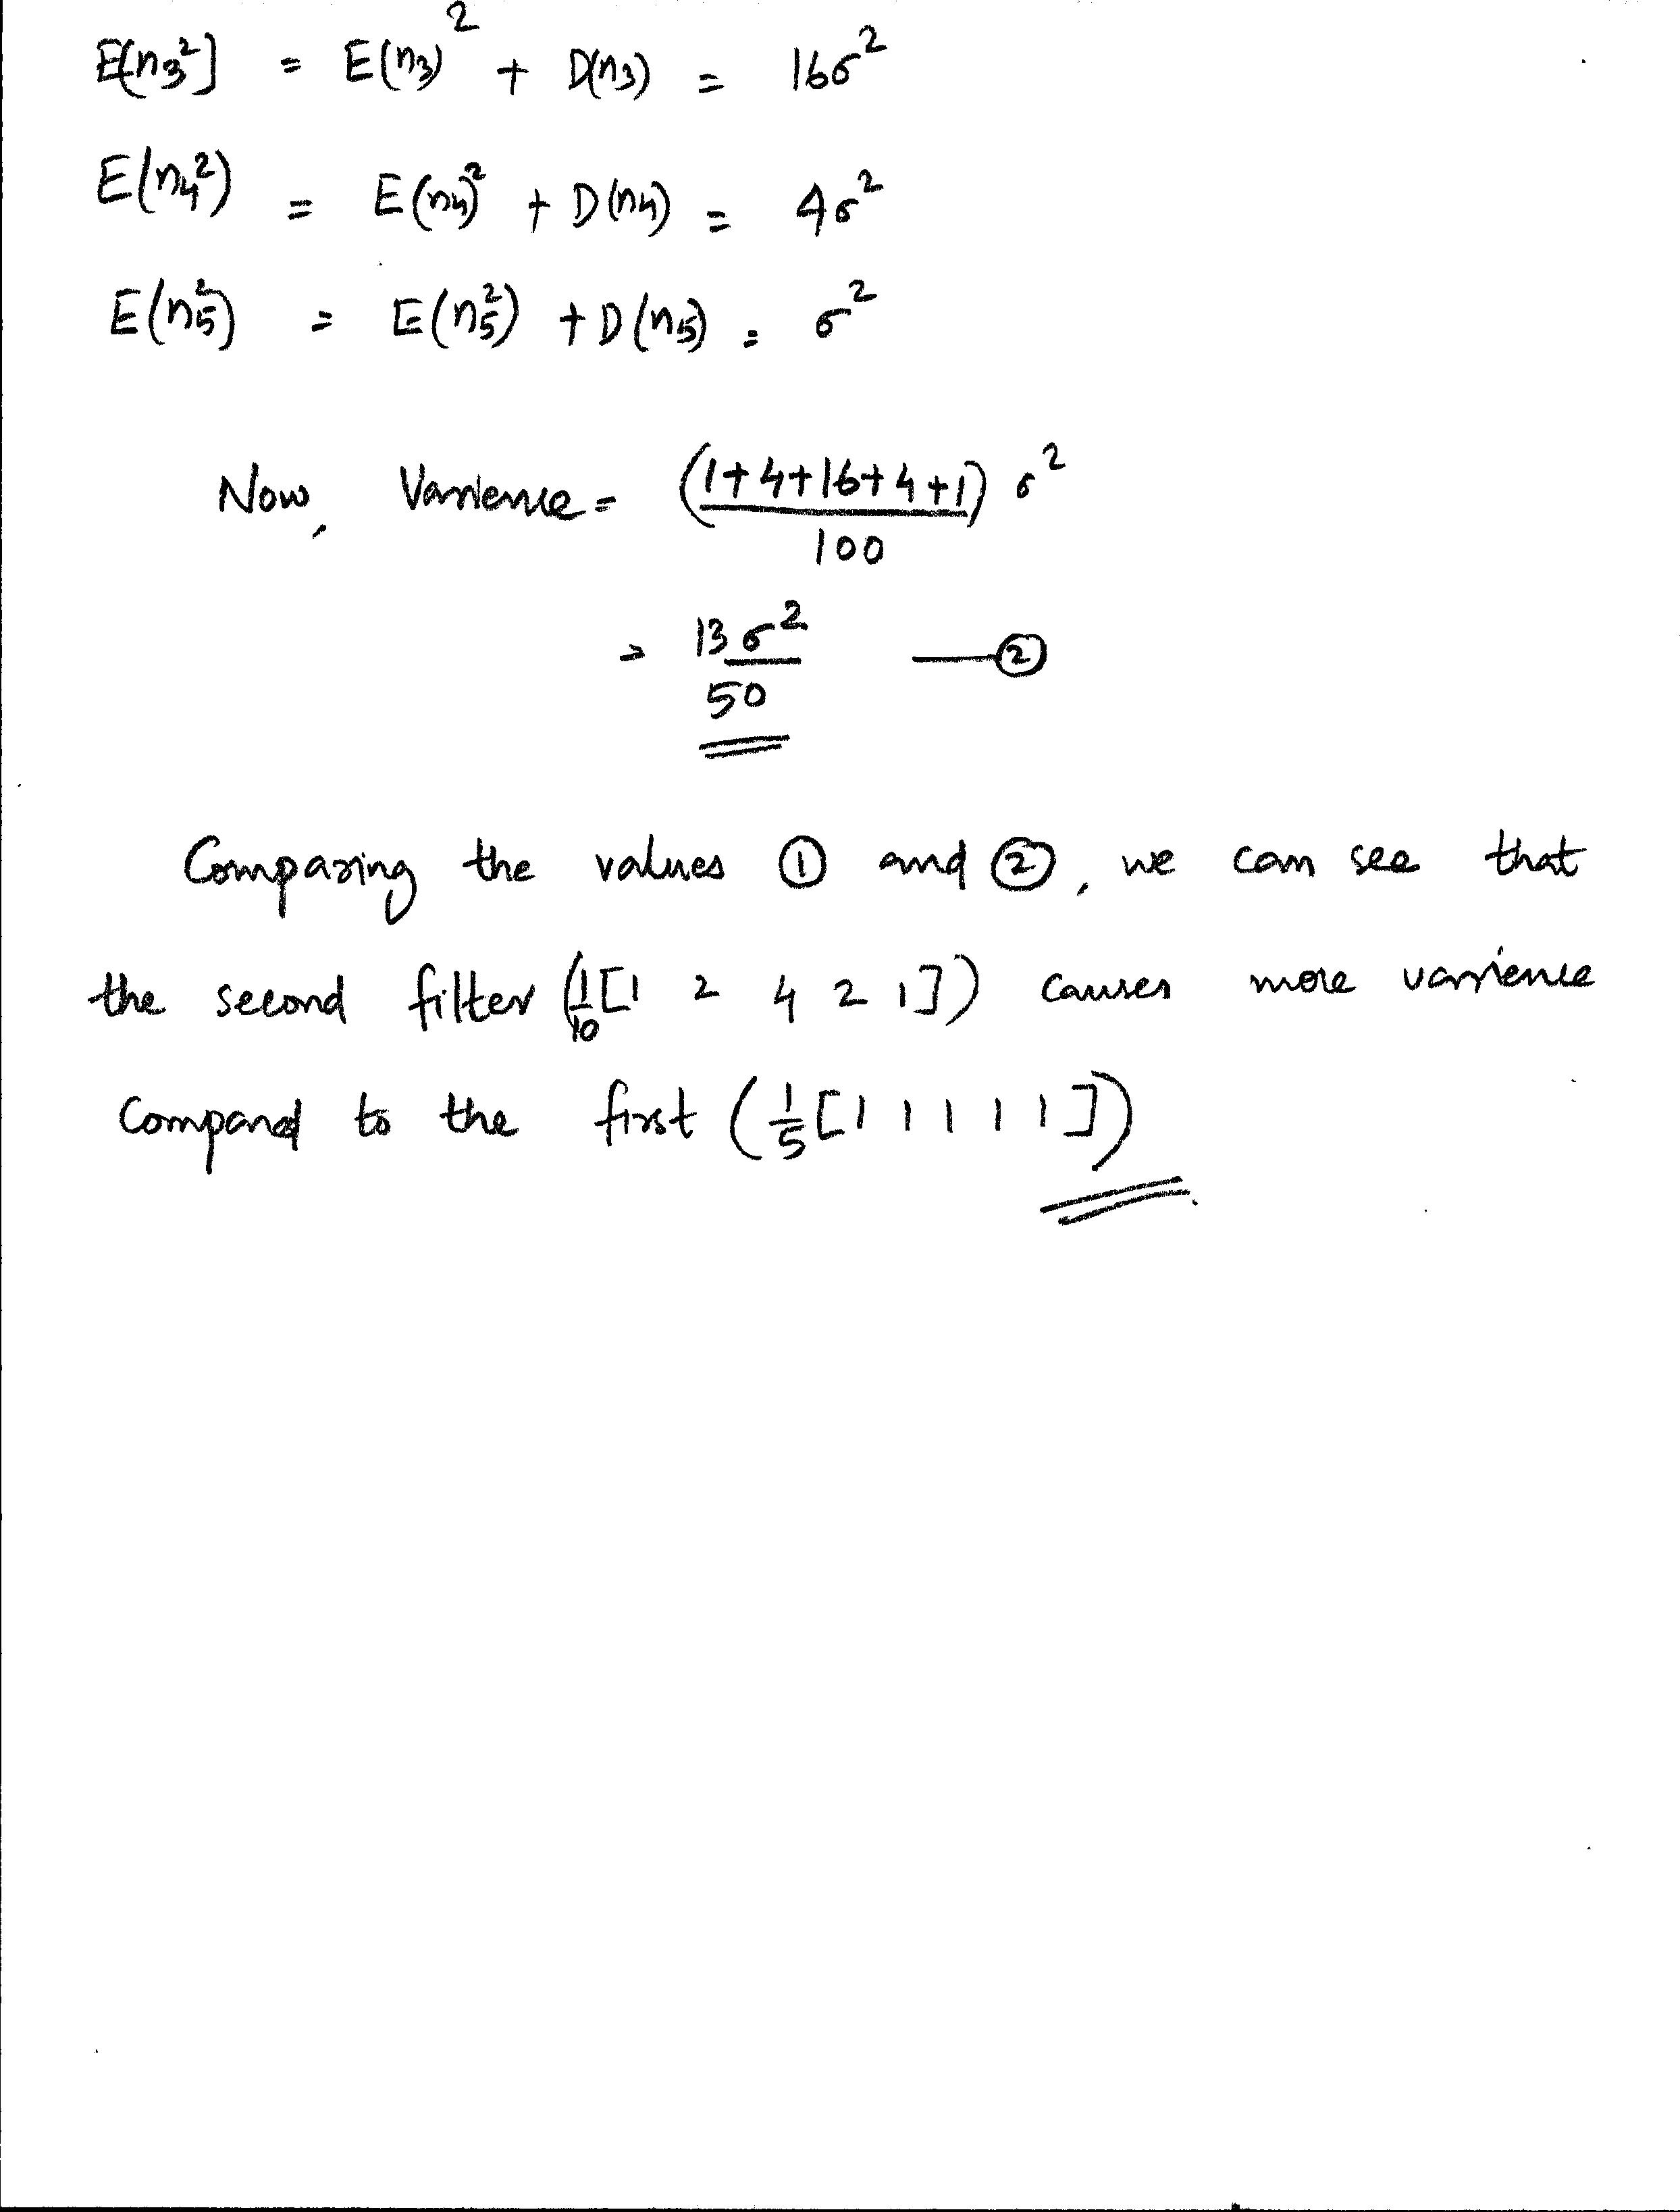
\includegraphics[width=15cm]{4.jpg}
\end{figure}

\begin{figure}
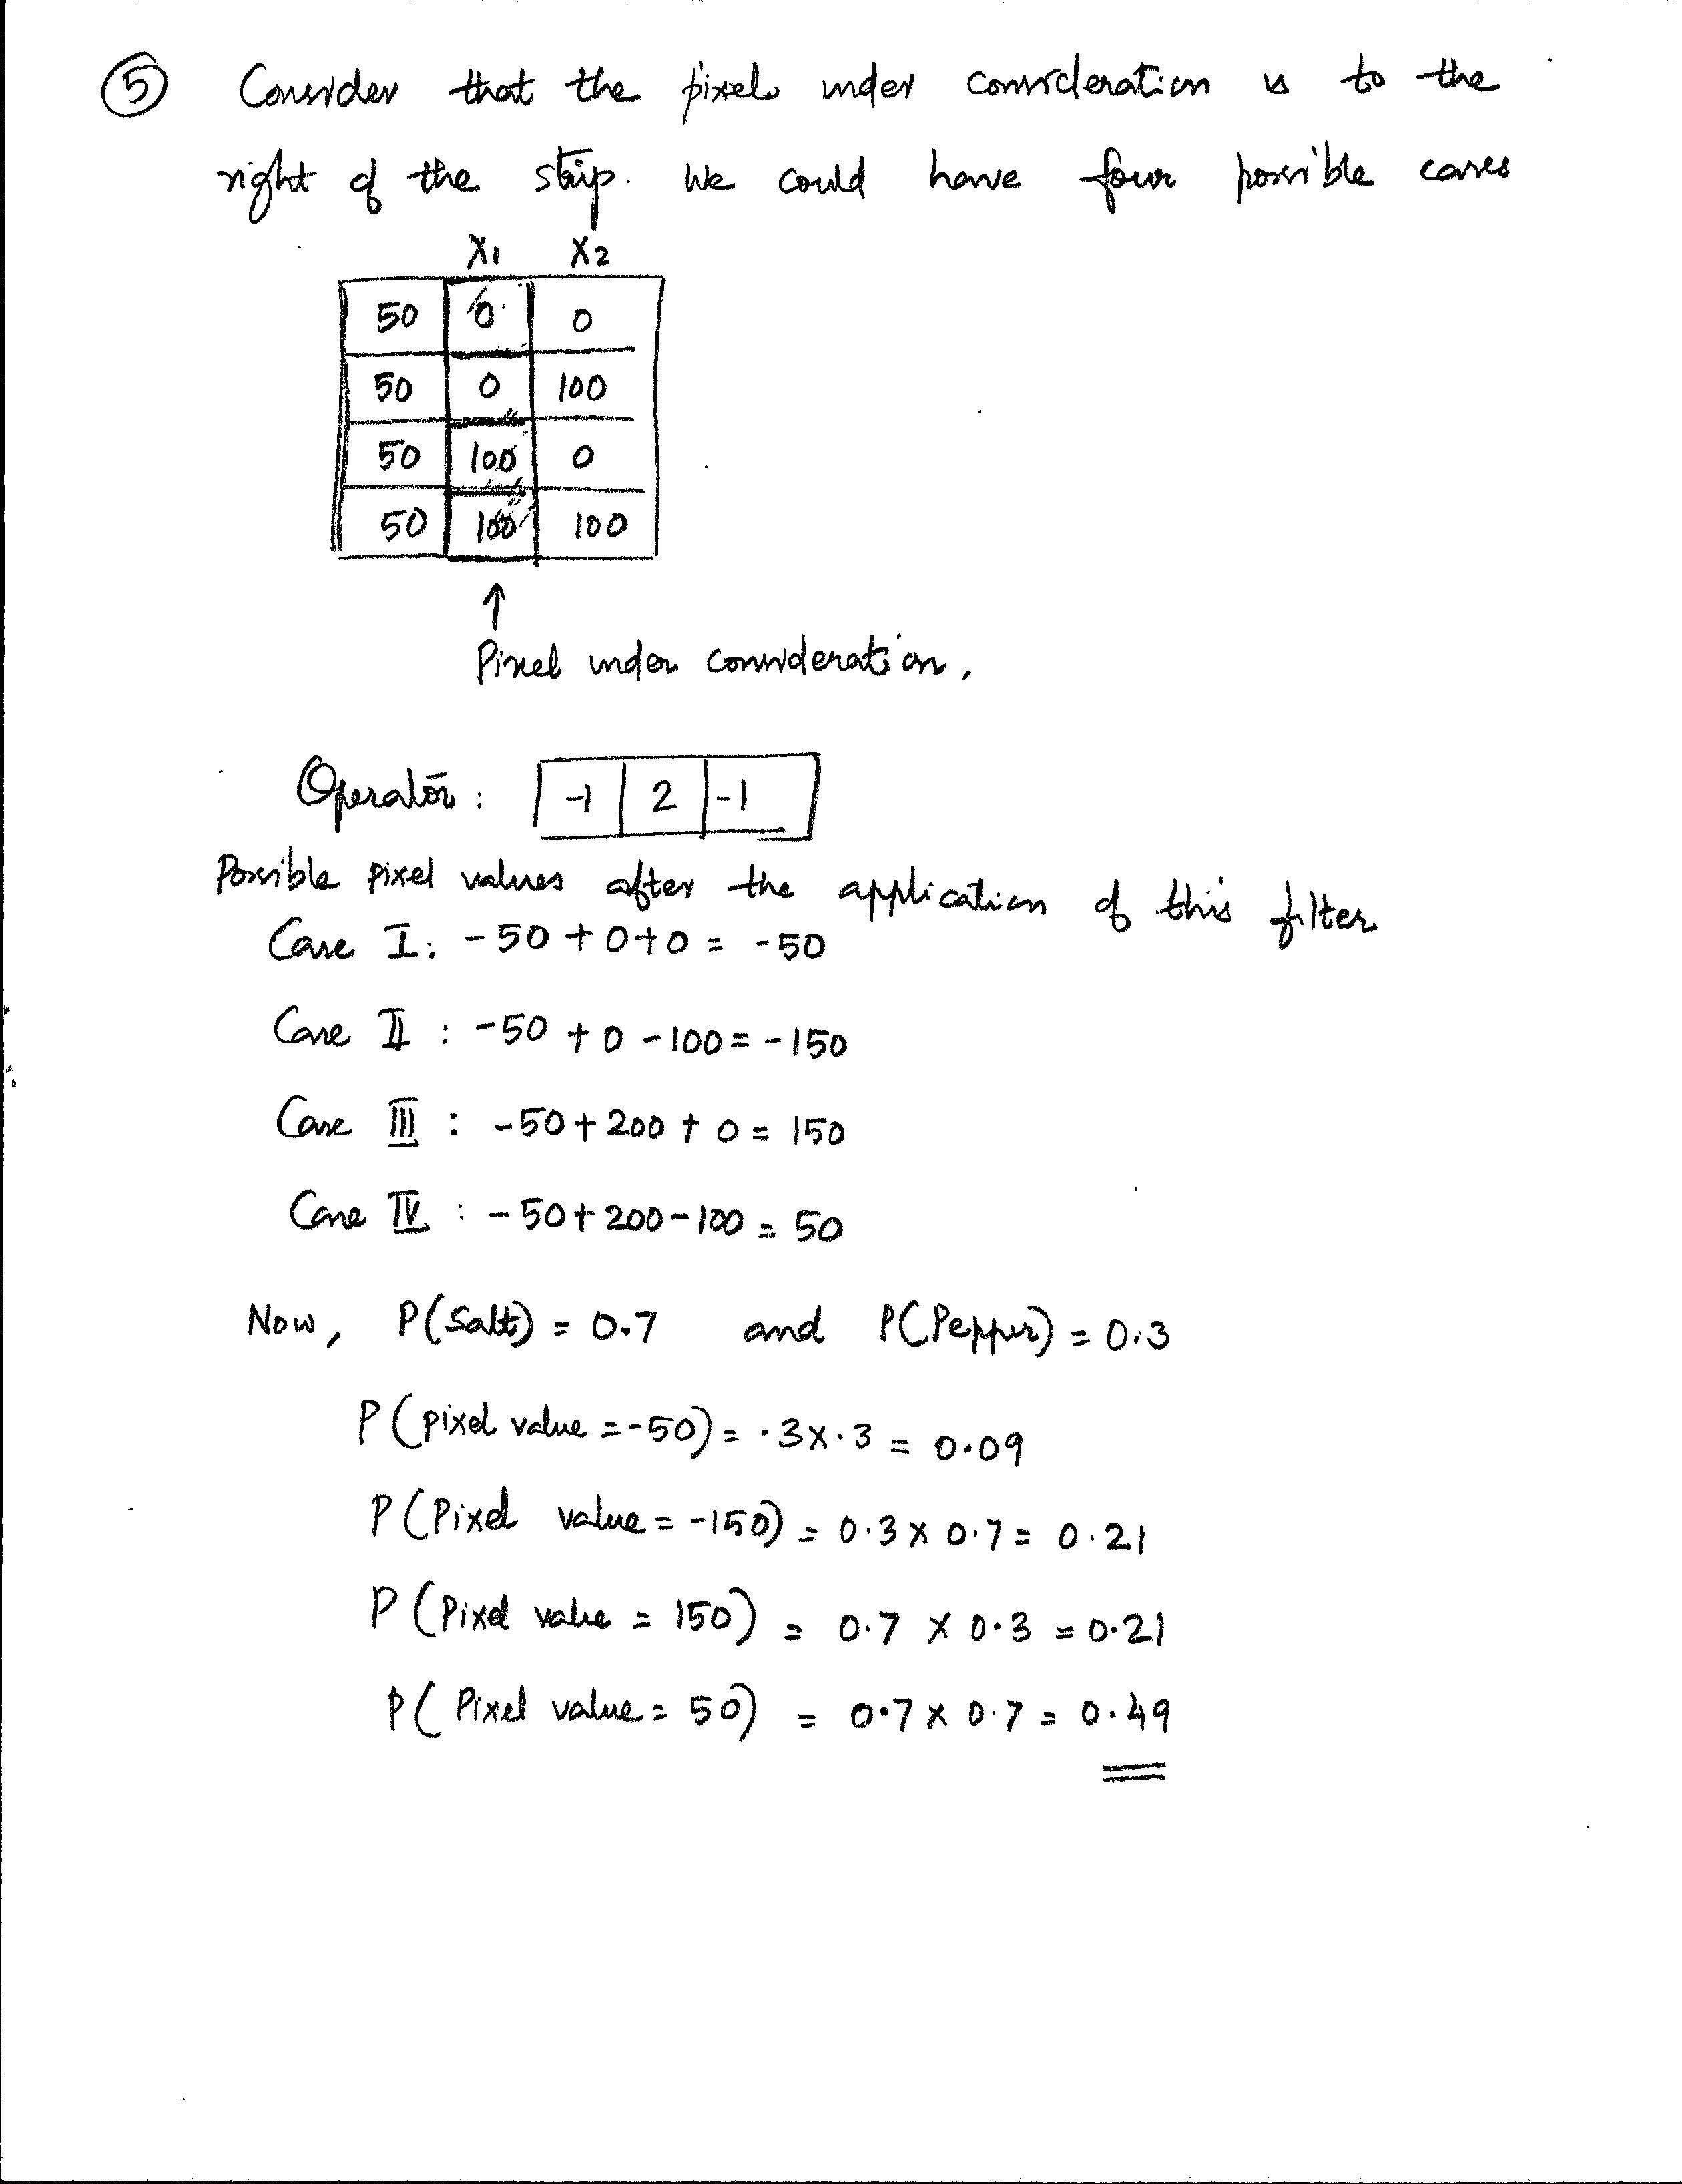
\includegraphics[width=15cm]{5.jpg}
\end{figure}

\begin{figure}
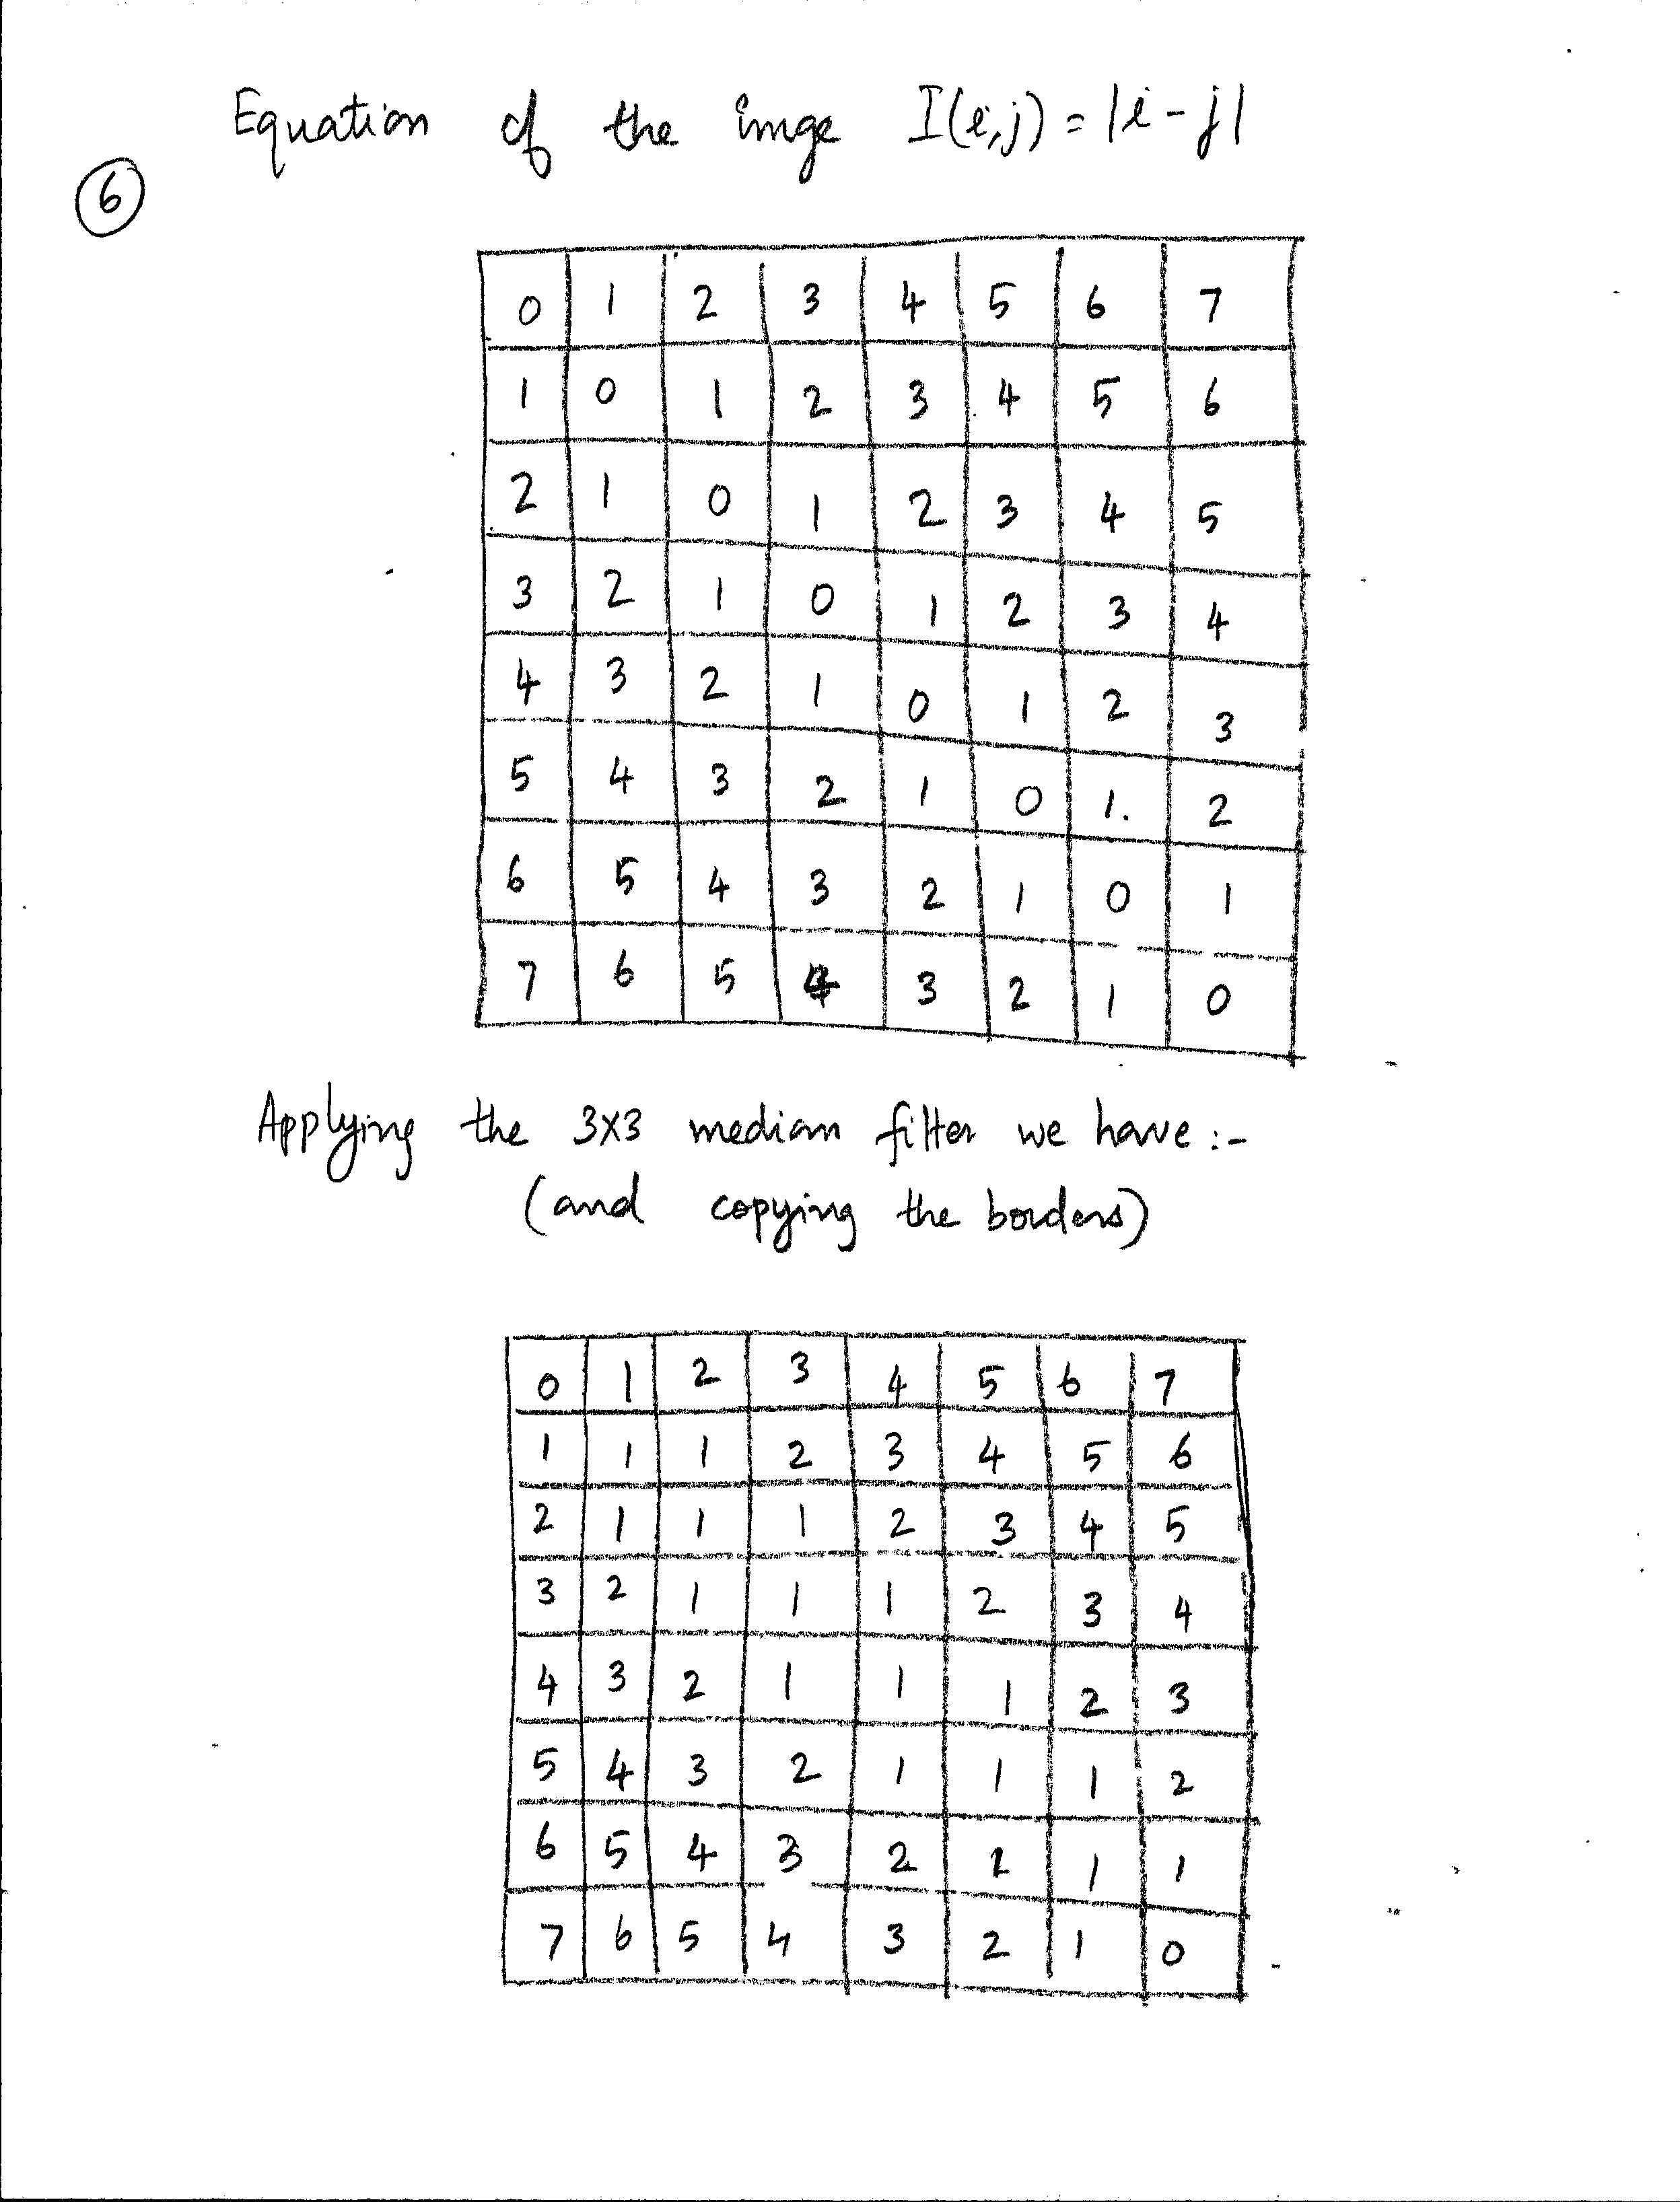
\includegraphics[width=15cm]{6.jpg}
\end{figure}

\begin{figure}
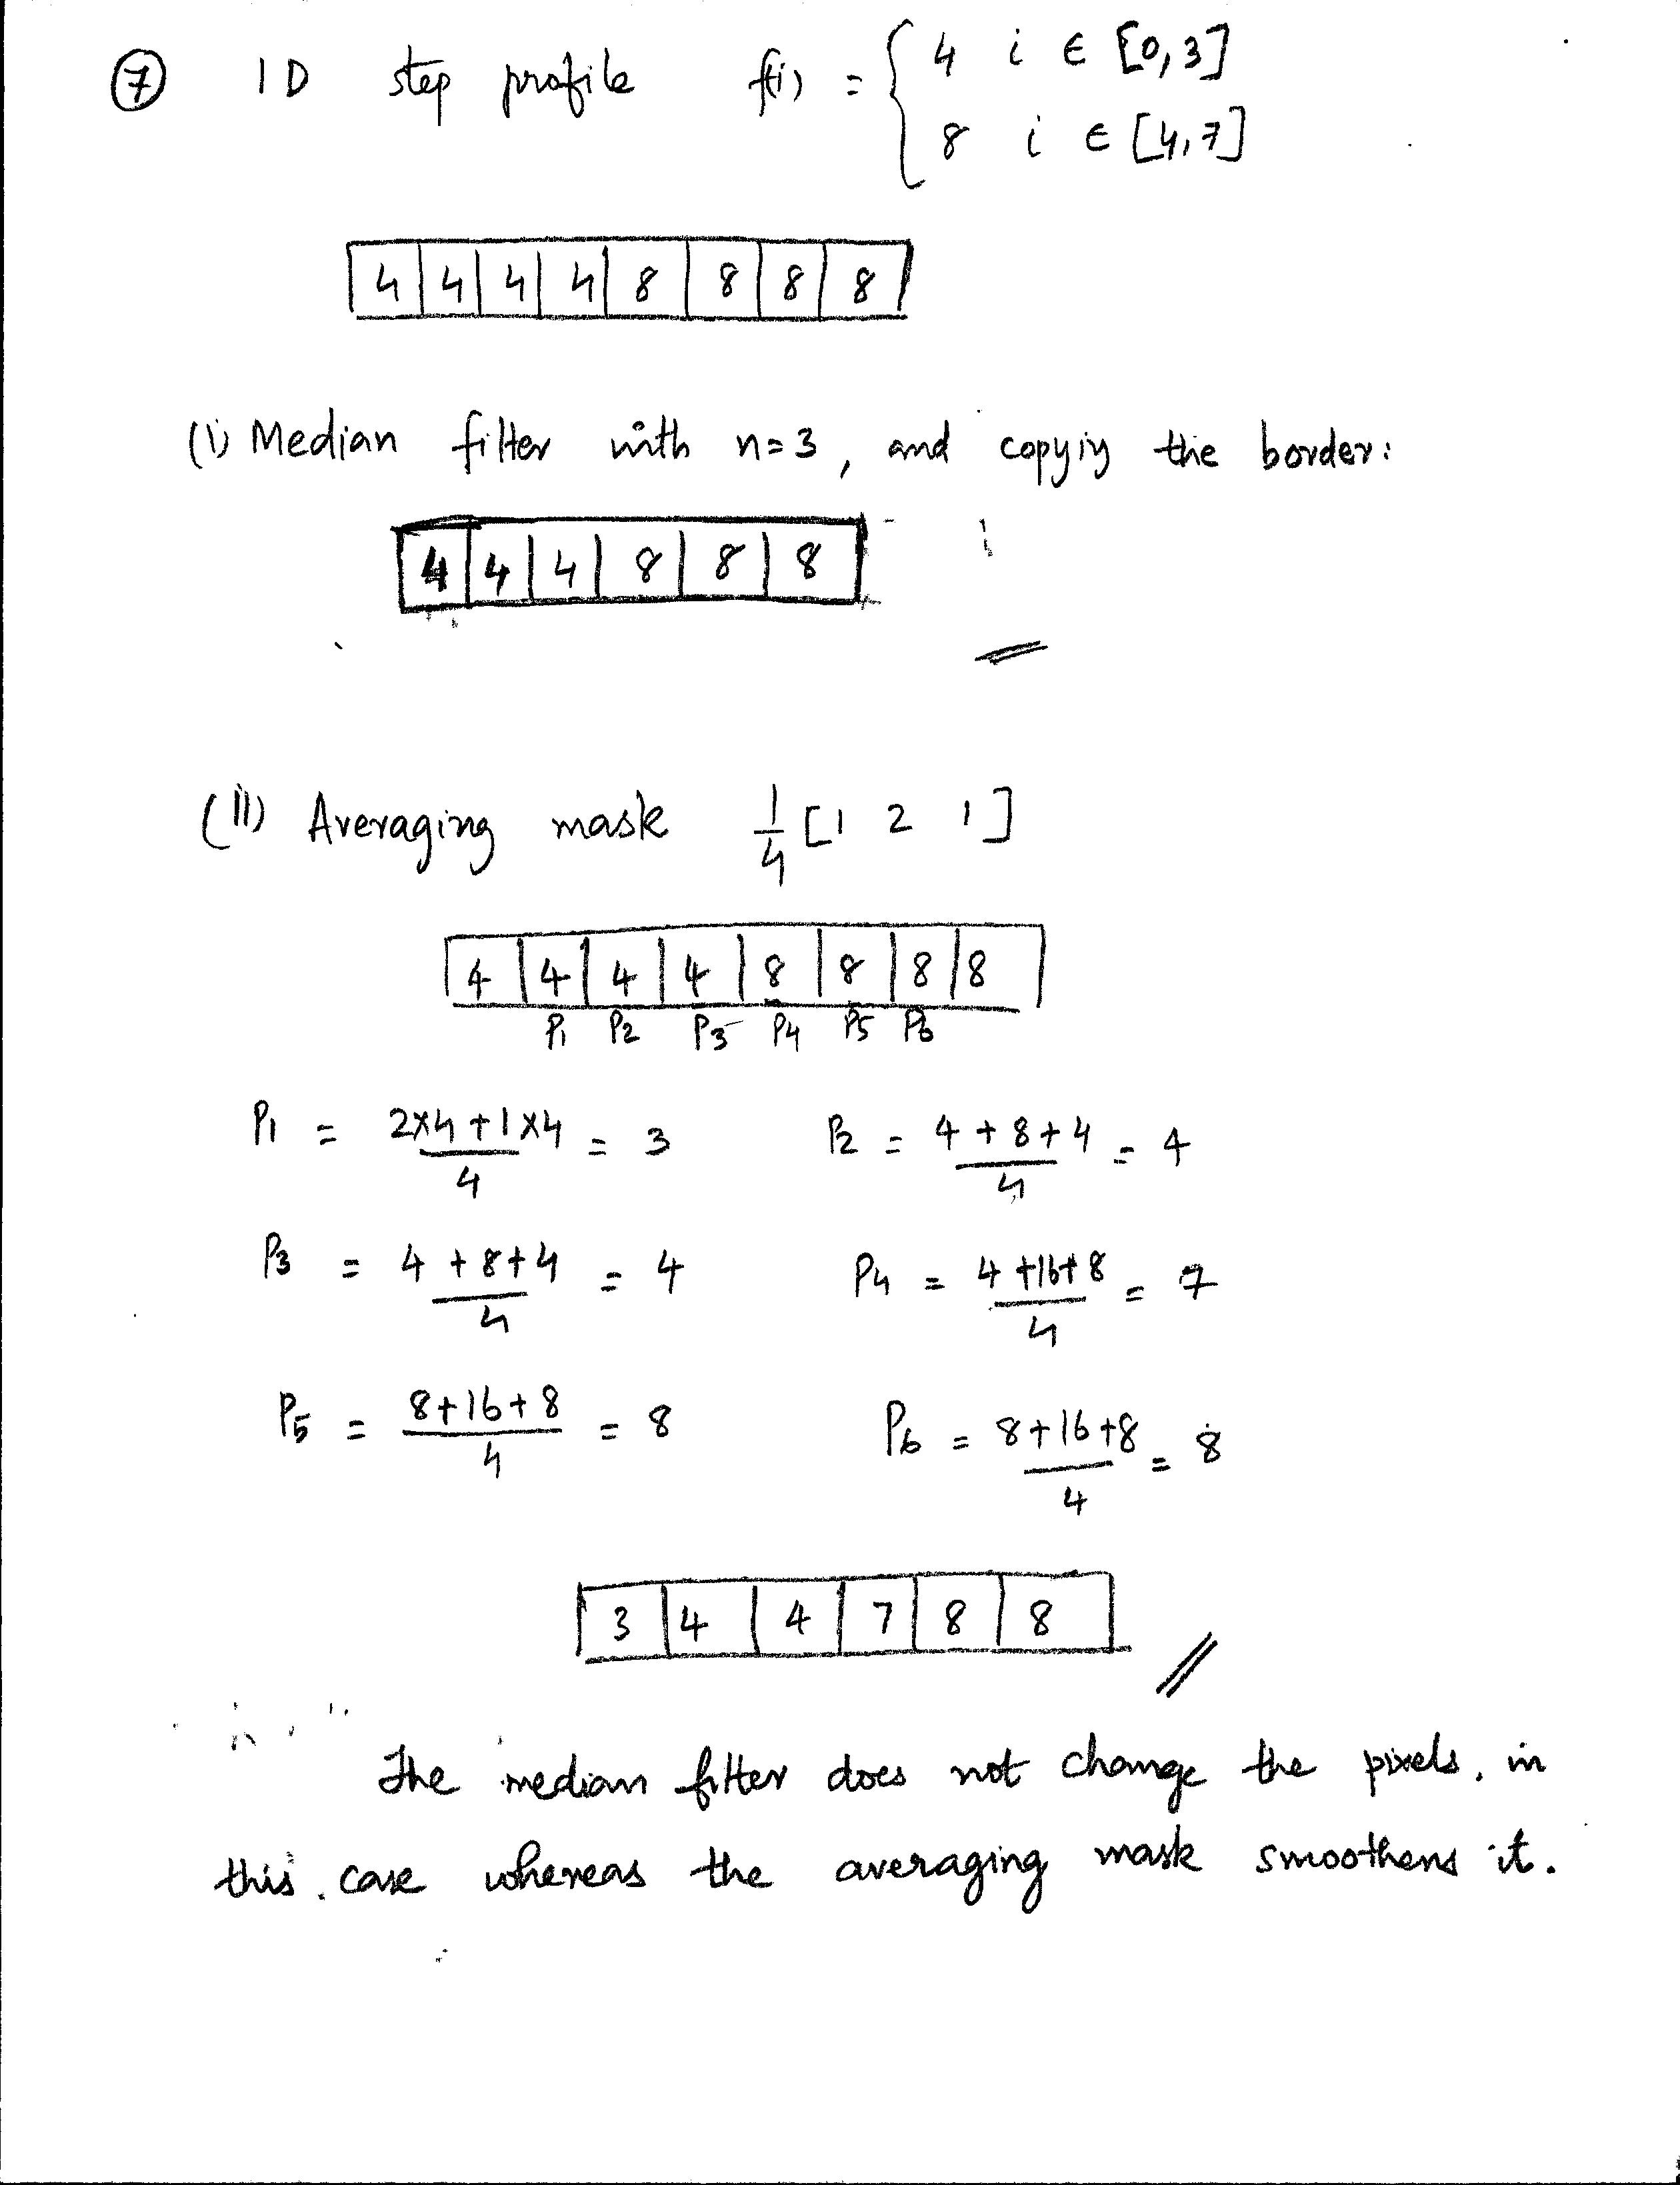
\includegraphics[width=15cm]{7.jpg}
\end{figure}


\end{document}


